% !TeX root = er.tex

\chapter{Robótica de enxame}\label{ch.swarm}

As fábricas utilizam vários robôs para alcançar objetivos como pintar e soldar um carro (Fig.\ref{fig.assemblyline}). O uso de vários robôs encurta o tempo de fabricação ao realizar diferentes tarefas simultaneamente, tais como soldar peças em ambos os lados de um carro. Estas tarefas são normalmente projetadas para serem independentes, sem nenhuma colaboração estreita entre os robôs. Mais tarde, os robôs, especialmente os robôs móveis, foram projetados para colaborar uns com os outros \emph{directly} para executar múltiplas ações simultaneamente em locais diferentes.

Aqui estão alguns exemplos de tarefas que requerem a colaboração de vários robôs:
\begin{itemize}
\item Manipular grandes elementos estruturais em edifícios, bem como em ambientes de difícil acesso para o ser humano, como no espaço ou debaixo d'água.
\item Realizando uma tarefa através da colaboração de diferentes tipos de robôs: em um desastre de grande escala, um drone voador pode localizar áreas onde é provável que as vítimas sejam encontradas, enquanto um robô rastreado no chão procura essas áreas, concentrando-se em lugares que podem estar escondidos da observação aérea por árvores ou escombros.
\item Realizar medições simultâneas em diferentes locais: medir distúrbios sonoros em diferentes partes de um edifício, ou monitorar a poluição após um acidente industrial. 
\end{itemize}
O que é comum nestas situações é que vários robôs participam da execução de uma tarefa e precisam se coordenar entre si porque estão agindo sobre o mesmo objeto físico, mesmo que não estejam próximos uns dos outros no ambiente. 

A colaboração entre robôs também pode ser usada para acelerar a execução de uma tarefa, fazendo com que vários robôs executem a tarefa em paralelo. Considere a possibilidade de medir a poluição em uma grande área: um único robô pode percorrer toda a área (como um aspirador robótico em um apartamento), mas a tarefa será realizada muito mais rapidamente se vários robôs dividirem as áreas a serem cobertas entre si.

\section{Abordagens para implementar a colaboração entre robôs}

Há duas abordagens principais para o projeto de sistemas compostos de vários robôs. A primeira é um sistema \textit{centralizado}, onde um componente central (um dos robôs ou um computador externo) coordena todos os robôs e suas tarefas. A vantagem de um sistema centralizado é que ele é relativamente simples de implementar. A principal desvantagem é que é difícil expandir porque adicionar mais robôs acrescenta carga de processamento à estação central onde toda a inteligência está concentrada. Em um sistema centralizado, os próprios robôs podem ser "mudos", mas a maioria dos robôs tem um poder de computação significativo que não é bem utilizado nesta arquitetura. Outra séria desvantagem de um sistema centralizado é que o componente central é um único ponto de falha. Se ele parar de funcionar, o sistema inteiro falha. Em ambientes críticos, é inaceitável empregar um sistema que não seja robusto sob a falha de um único componente.

Se olharmos para o mundo animal, vemos que muitas atividades são \emph{distribuídas}, ou seja, indivíduos independentes trabalham juntos para atingir objetivos comuns de toda a população. As formigas otimizam seu caminho para as fontes de alimento não dependendo de uma formiga para despachar outras para procurar e depois processar as informações devolvidas, mas por um esforço distribuído de toda a colônia de formigas. As formigas individuais marcam o solo com feromônios que são percebidos pelas outras formigas. Se algumas formigas são comidas por um predador, o resto da colônia sobrevive, assim como o conhecimento encarnado nos locais das feromonas. A eficiência e robustez desta abordagem foi demonstrada nos algoritmos do Cap.~\ref{ch.obstacle}.

\emph{Swarm robotics} é uma abordagem distribuída da robótica que tenta coordenar o comportamento copiando mecanismos inspirados no comportamento dos animais sociais. Estes mecanismos, muitas vezes locais e simples, permitem que um grupo alcance um desempenho global que não poderia ser alcançado por um indivíduo por si só. Os sistemas distribuídos têm as seguintes vantagens:
\begin{itemize}
\item Eles são robustos. Perder um em cada dez robôs apenas reduz o desempenho do sistema em cerca de dez por cento, ao invés de causar falhas em todo o sistema.
\item Eles são flexíveis e escaláveis. O número de robôs pode ser adaptado à tarefa. Se houver dez robôs no sistema, mas cinco são suficientes para realizar a tarefa, os outros cinco podem ser atribuídos a outras tarefas, enquanto que se dez robôs não puderem realizar a tarefa eficientemente, outros dez podem ser facilmente adicionados.
\end{itemize}
Estas vantagens se dão ao custo do esforço necessário para projetar e implementar a coordenação entre os robôs. Na robótica de enxame, assim como na natureza, existem mecanismos de coordenação relativamente simples que viabilizam sistemas distribuídos.

Este capítulo apresenta duas abordagens para a coordenação em robótica de enxame:
\begin{itemize}
\item Coordenação baseada em informações (Sec.~\ref{s.swarm-info}), onde a interação é na forma de comunicação entre robôs. Isto pode ser feito ou diretamente, passando mensagens eletrônicas explicitamente ou indiretamente, colocando mensagens no ambiente.
\item Coordenação física (Sec.~\ref{s.swarm-physical}), onde robôs individuais interagem no nível mecânico, seja diretamente exercendo forças uns sobre os outros ou indiretamente manipulando um objeto comum.
\end{itemize}

\section{Coordenação por intercâmbio local de informações}\label{s.swarm-info}

As comunicações podem ser tanto globais quanto locais. Suponha que você receba uma ligação de seus amigos e eles o informem: ``Vemos uma sorveteria à esquerda''. Esta informação \emph{global} é inútil a menos que eles lhe informem sua localização atual. Entretanto, se você estiver caminhando lado a lado com eles e alguém disser: ``Vejo uma sorveteria à esquerda'', a partir desta informação \emph{local} você imediatamente sabe a localização aproximada da loja e pode facilmente localizá-la visualmente.

Inspirada pela natureza, a robótica do enxame utiliza comunicações locais dentro de uma arquitetura distribuída. Algumas zebras nas bordas externas de um rebanho procuram por predadores e sinalizam os outros por som ou movimento. O pastoreio é uma estratégia de sobrevivência bem sucedida para os animais porque as comunicações locais permitem que um grande número de animais fuja imediatamente após a detecção de um predador por um pequeno número de observadores de alerta.

\subsection{Comunicações diretas}

\emph{Direto} o intercâmbio local de informações é alcançado quando um amigo fala com você. Os animais não falam, mas usam tanto o som quanto o movimento e o contato físico para conseguir uma troca de informações local direta. Os robôs implementam comunicações locais diretas eletronicamente (como WiFi local ou Bluetooth), ou transmitindo e recebendo luz ou som. Alternativamente, eles podem usar uma câmera para detectar mudanças em outro robô, como acender uma luz. 

As comunicações locais podem ser \emph{direcionais} ou \emph{não direcionais}. Comunicações via rádio como Bluetooth são locais (apenas alguns metros) e geralmente o robô receptor não tenta determinar a direção para o robô transmissor. As comunicações direcionais locais podem ser implementadas usando uma fonte de luz como transmissor e um detector de abertura estreita ou uma câmera como receptor.

\subsection{Comunicações indiretas}

\emph{Indireto} comunicações locais refere-se às comunicações através de um meio que pode armazenar uma mensagem transmitida para acesso posterior. O exemplo mais familiar é o correio, seja e-mail ou correio normal, onde o transmissor compõe a mensagem e a envia, mas a mensagem permanece no servidor ou nos correios até ser entregue ao receptor que, por sua vez, não pode acessá-la imediatamente. As comunicações indiretas em animais são chamadas \emph{stigmergy}; os animais deixam mensagens através do depósito de substâncias químicas que outros animais podem sentir. Mencionamos o uso de feremonas por formigas; outro exemplo é o uso da urina por um cão para marcar seu território.

As mensagens químicas são difíceis de implementar em robôs, mas os robôs podem deixar marcas óticas no chão como fizemos no algoritmo que simula uma colônia de formigas em busca de uma fonte de alimento (Sect.~\ref{s.ant-like-algo}). Lá foi usado apenas um robô, mas os algoritmos poderiam ser facilmente implementados com vários robôs porque é a marcação que é importante, não a identidade do robô que criou a marcação.

As comunicações indiretas também podem ser implementadas através da colocação ou manipulação de objetos no ambiente. Os aspiradores robóticos usam \emph{beacons} que podem ser colocados na entrada das salas que o robô deve evitar. É possível conceber balizas que registram quando uma sala já foi limpa e estas informações são (indiretamente) comunicadas a outros aspiradores de pó.

\emph{Karel the Robot} é um ambiente usado para ensinar programação. Os comandos movem um robô virtual em torno de uma grade na tela de um computador e o robô pode depositar e sentir "beepers" colocados em quadrados da grade (Fig.~\ref{fig.karel}).\footnote{A imagem é tirada da implementação do primeiro autor de Karel, o Robô em Raspadinha (\url{https://scratch.mit.edu/studios/520857}).}

\begin{figure}
\begin{center}
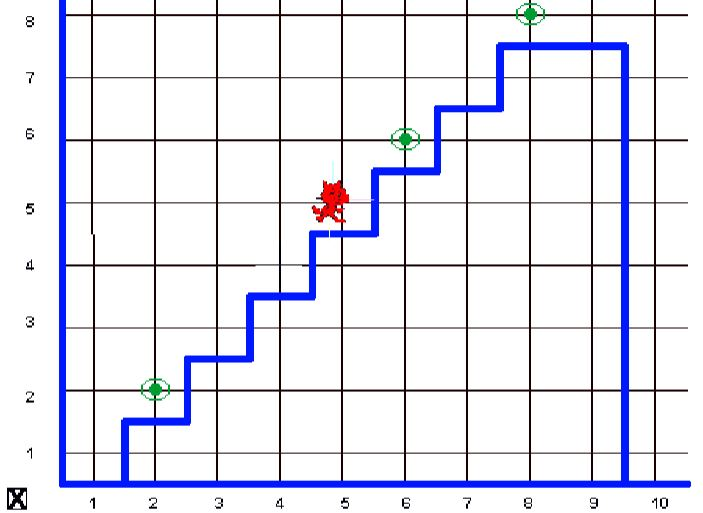
\includegraphics[width=.8\textwidth]{karel}
\end{center}
\caption{Karel o robô implementado em Scratch; os pontos verdes são os bipes}\label{fig.karel}
\end{figure}

As comunicações indiretas quando combinadas com a manipulação podem gerar padrões interessantes. A figura~\ref{fig.coll1} mostra um ambiente cheio de pequenos objetos e cinco robôs móveis equipados com garras. Os robôs seguem um conjunto simples de regras:
\begin{itemize}
\item Se o robô encontra um objeto isolado, ele pega o objeto;
\item Se o robô encontrar um objeto isolado mas já estiver segurando um, ele coloca o novo objeto ao lado do que foi encontrado;
\item O robô evita paredes e grupos de vários objetos.
\end{itemize}
Parece que estas regras farão com que os robôs acabem colocando todos os objetos em grupos de dois, mas isto não acontece como mostrado na Fig.~\ref{fig.coll2}. A razão é que um grupo de objetos \emph{visto de lado} pode parecer um objeto isolado, então um objeto adicional é colocado no grupo. O resultado é que grandes grupos de objetos são montados puramente por comunicação indireta.

\begin{figure}
\begin{minipage}{.45\textwidth}
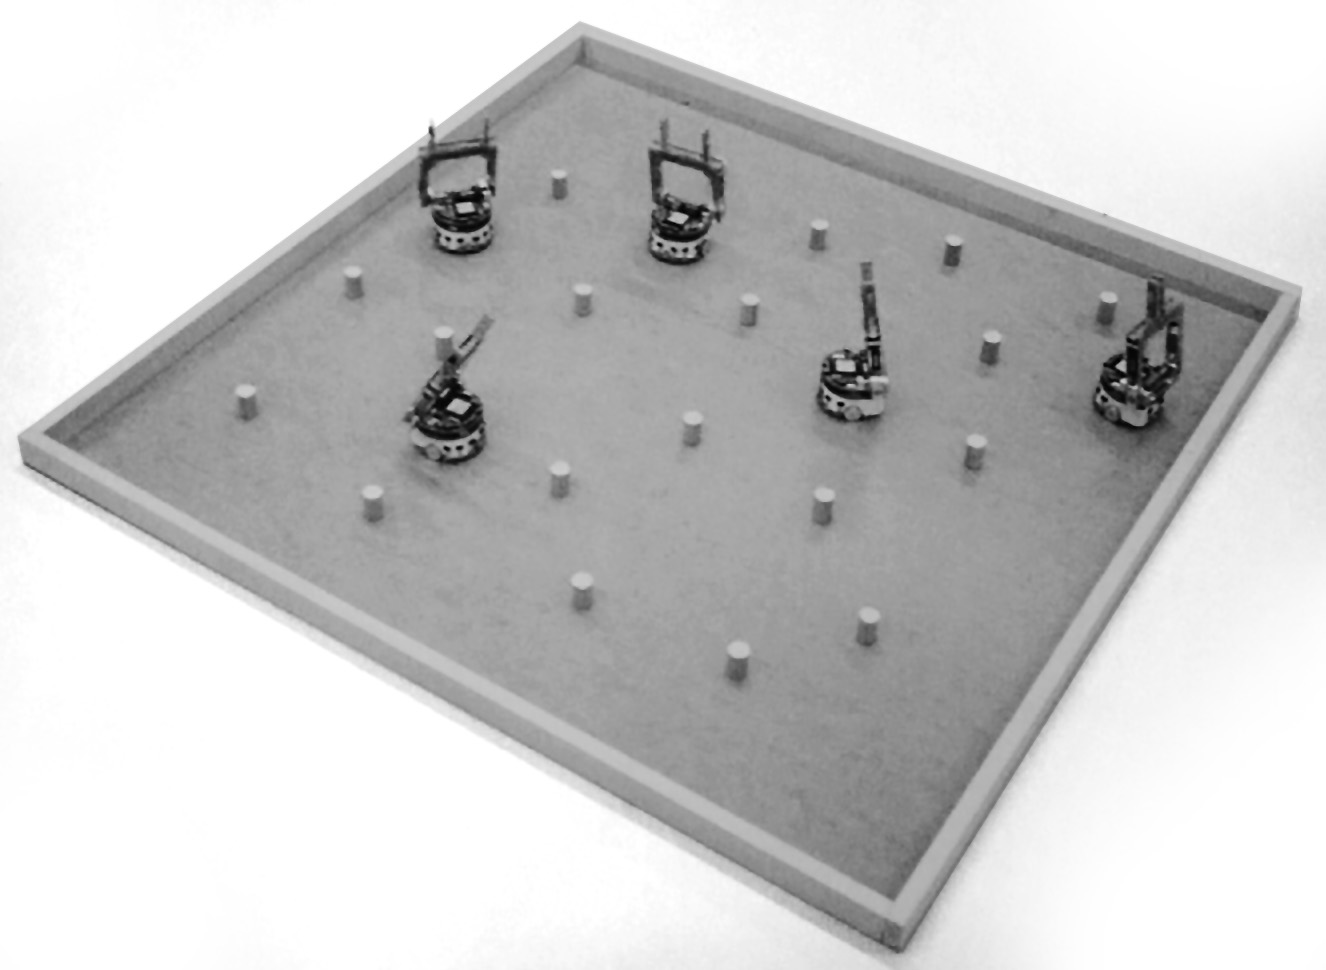
\includegraphics[width=.45\textwidth]{coll1}
\caption{Robôs garras em um ambiente repleto de pequenos objetos}
\label{fig.coll1}
\end{minipage}
\hspace{\fill}
\begin{minipage}{.45\textwidth}
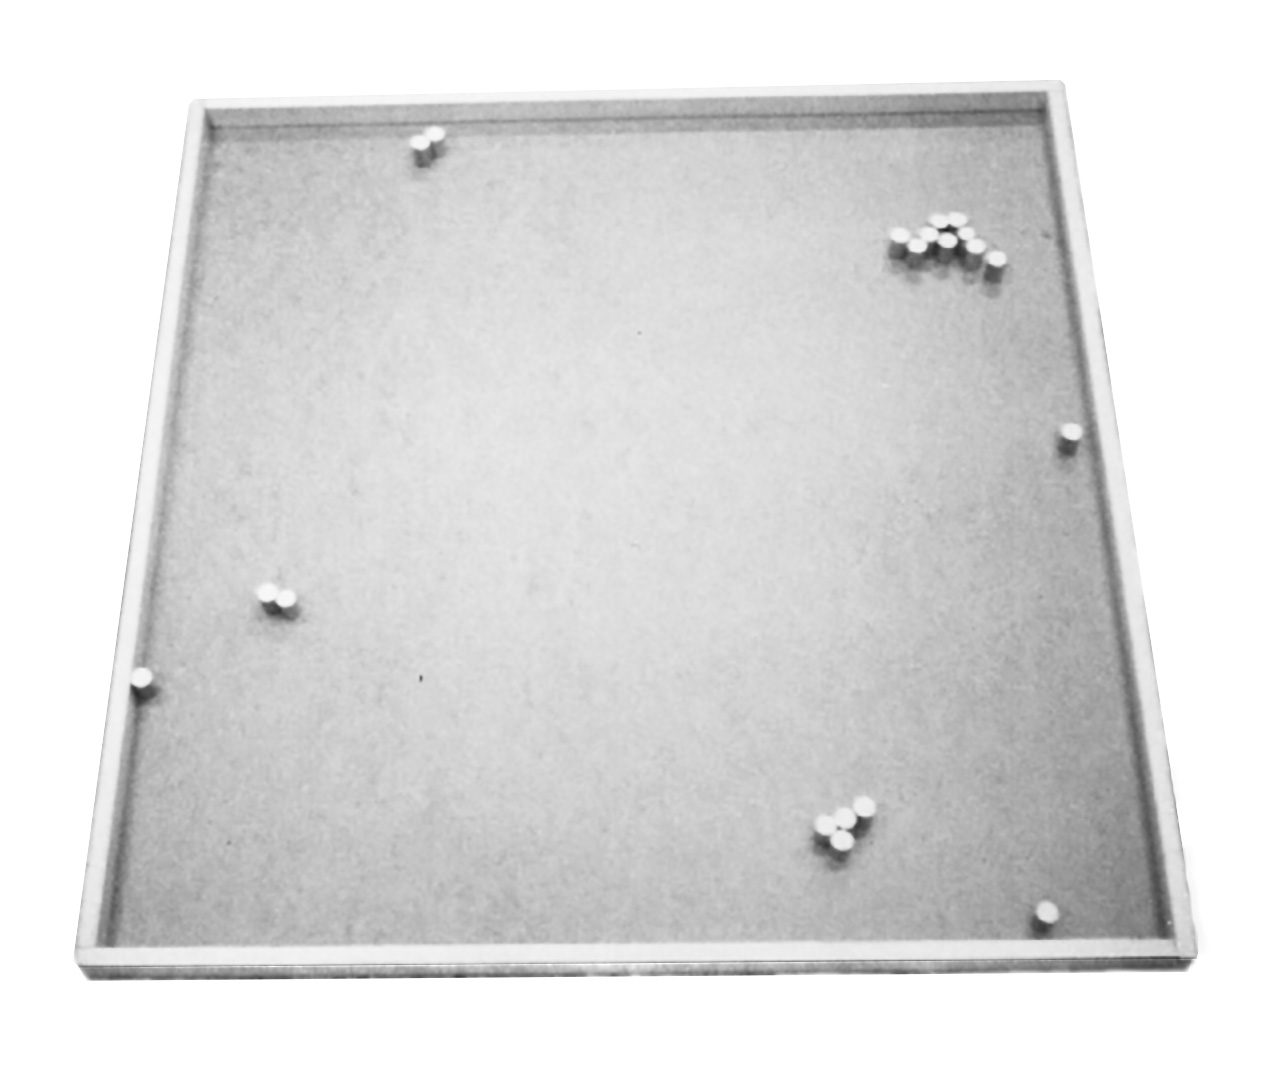
\includegraphics[width=.45\textwidth]{coll2}
\caption{Os objetos foram coletados em grupos}
\label{fig.coll2}
\end{minipage}
\end{figure}

%\begin{figure}
%\subfigures
%\begin{minipage}{\textwidth}
%\leftfigure{
%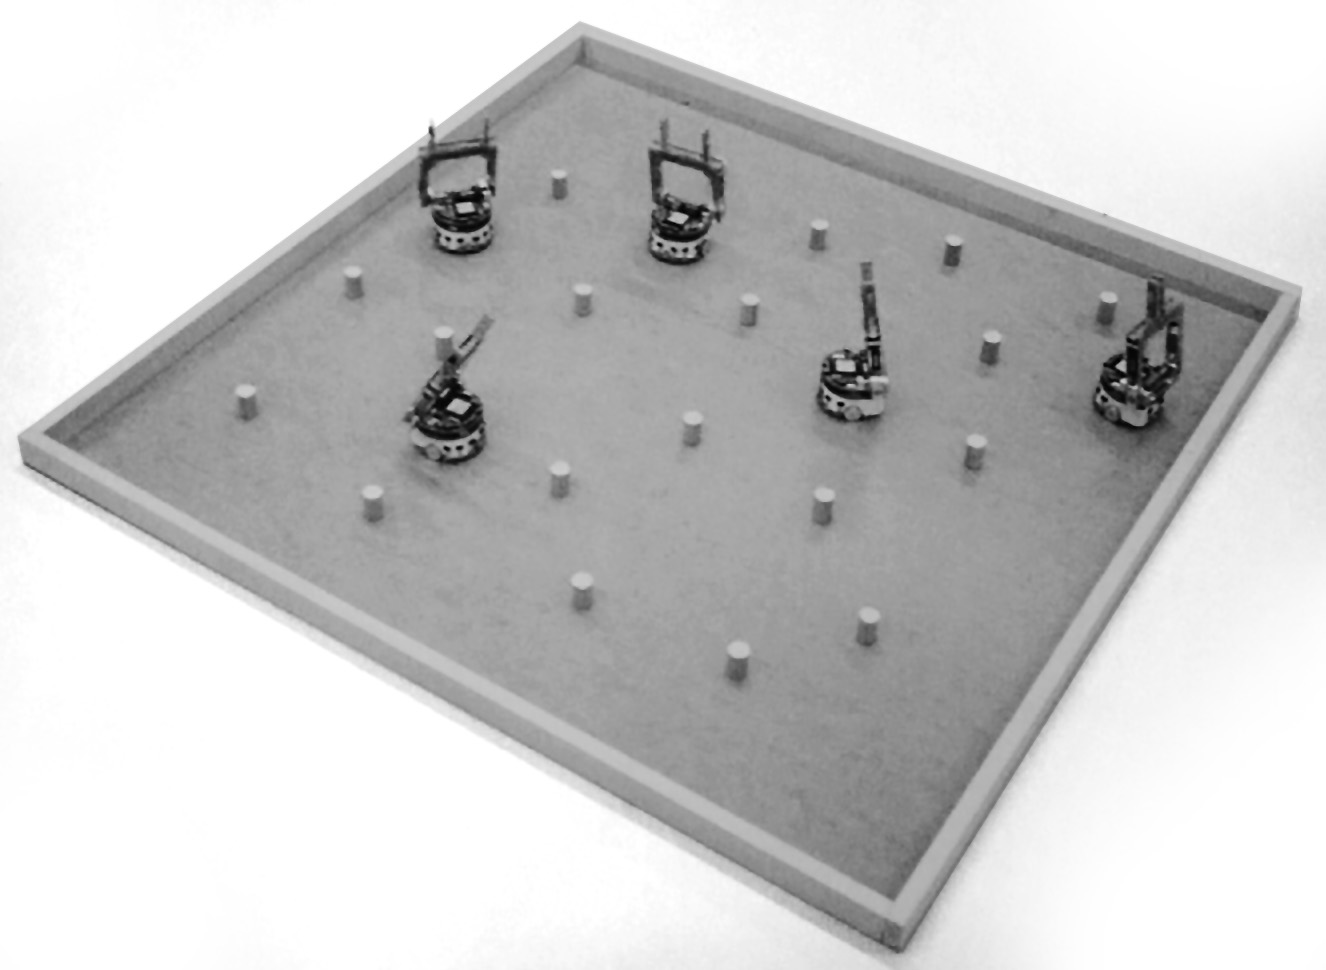
\includegraphics[width=.45\textwidth]{coll1}
%}
%\hspace{\fill}
%\rightfigure{
%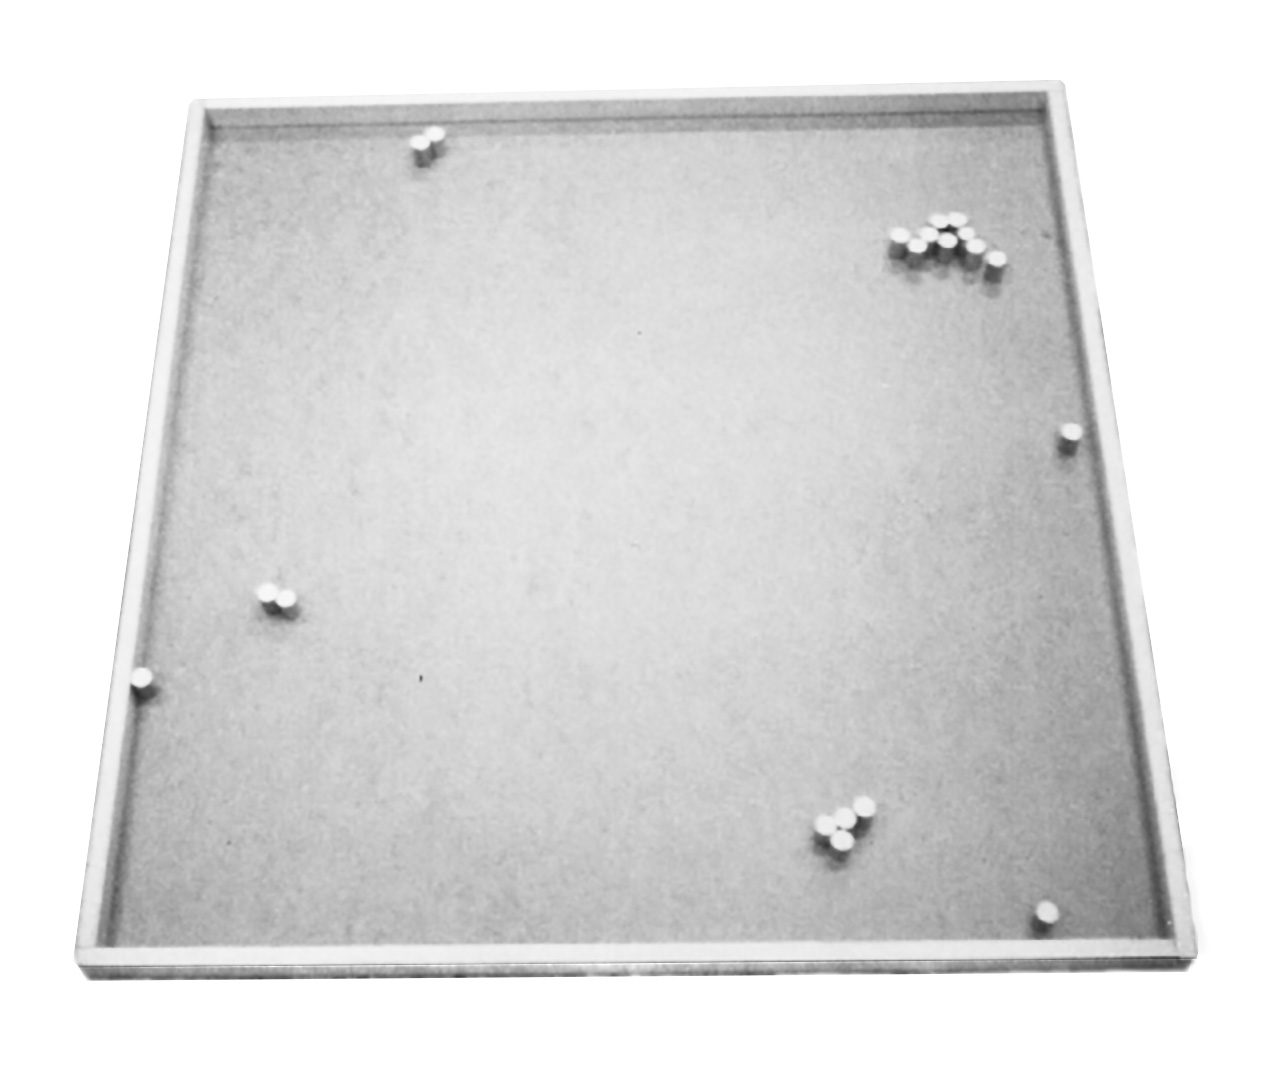
\includegraphics[width=.45\textwidth]{coll2}
%}
%\leftcaption{Gripper robots in an environment filled with small objects}\label{fig.coll1}
%\rightcaption{The objects have been collected into groups}\label{fig.coll2}
%\end{minipage}
%\end{figure}

\subsection{O algoritmo BeeClust}

O algoritmo BeeClust é um algoritmo de enxame inspirado no comportamento das abelhas. Ele usa uma arquitetura distribuída e comunicações locais para gerar um resultado global. O algoritmo BeeClust é baseado na forma como abelhas muito jovens se aglomeram em torno de locais de temperatura ótima na escuridão de seu ninho. Eles medem temperaturas locais e detectam colisões com outras abelhas.  O algoritmo pode ser usado por um enxame de robôs para localizar a poluição; em vez de medir a temperatura, cada robô mede alguma quantidade física que indica os níveis de poluição. Com o tempo, os robôs se reunirão em grupos em locais de altos níveis de poluição.

A figura~\ref{fig.beeclust} mostra uma máquina estatal implementando o algoritmo. O robô se move aleatoriamente até atingir outro robô, quando mede a temperatura no local da colisão. Ele espera neste local por um período de tempo proporcional à temperatura que encontrou e depois volta a se mover aleatoriamente. Quando o robô se move, ele evita obstáculos como as paredes. O algoritmo usa o que talvez seja a forma mais simples de comunicação: a detecção de uma colisão com outro robô. A natureza localizada das comunicações é essencial para o correto funcionamento do algoritmo.

\begin{figure}
\begin{center}
\begin{tikzpicture}[node distance = 4cm and 5cm,align=left,minimum size=16mm,every loop/.style={min distance=16mm}]
% Nodes
\node[draw,circle] (moving) {\p{moving}};
\node[draw,circle] (waiting) [right=of moving] {\p{waiting}};
% Initial state arrow
\draw[->] (-15mm,10mm) to node [above left,yshift=-3mm] {\p{true} $\leadsto$ \p{fwd}} (moving);
% Transitions from moving
\path[->] (moving) edge [loop above] node [above,yshift=-4mm] {\p{collision with wall} $\leadsto$ \p{turn randomly, fwd}} ();
\path[->] (moving) edge node[above] {\p{collision with robot} $\leadsto$\\ \p{measure temperature,}\\\p{calculate waiting time}} (waiting);
% Transitions from waiting
\path[->,bend left=20] (waiting) edge node[below,yshift=3mm] {\p{wait expired} $\leadsto$ \p{turn randomly, fwd}} (moving);
\end{tikzpicture}
\end{center}
\caption{Algoritmo BeeClust}\label{fig.beeclust}
\end{figure}

Inicialmente, os robôs colidirão em locais aleatórios, mas aqueles que estão em locais com temperaturas mais altas permanecerão lá por períodos mais longos, o que, por sua vez, causará colisões adicionais. A longo prazo, a maioria dos robôs formará um aglomerado na área com as temperaturas mais altas. Eles colidem uns com os outros com freqüência, já que estar em uma multidão aumenta o número de colisões. É claro que este mecanismo só pode funcionar com um grande número de robôs que geram muitas colisões que levam a numerosas medidas e aglomerações. 

\subsection{A implementação ASSISIbf de BeeClust}

Dentro do projeto ASSISIbf, pesquisadores da Universidade de Graz utilizaram robôs Thymio para implementar o algoritmo BeeClust como parte da pesquisa sobre o comportamento das abelhas em um ninho. O algoritmo simula um grupo de abelhas jovens em uma arena circular fria, onde duas fontes virtuais de calor são colocadas à direita e à esquerda da arena. Inicialmente, apenas uma dessas fontes de calor está ativa. As fontes de calor são simuladas por dois grupos de três robôs nas bordas da arena. (Fig.~\ref{fig.beeclust-demo}(a)).

\begin{figure}
\begin{center}
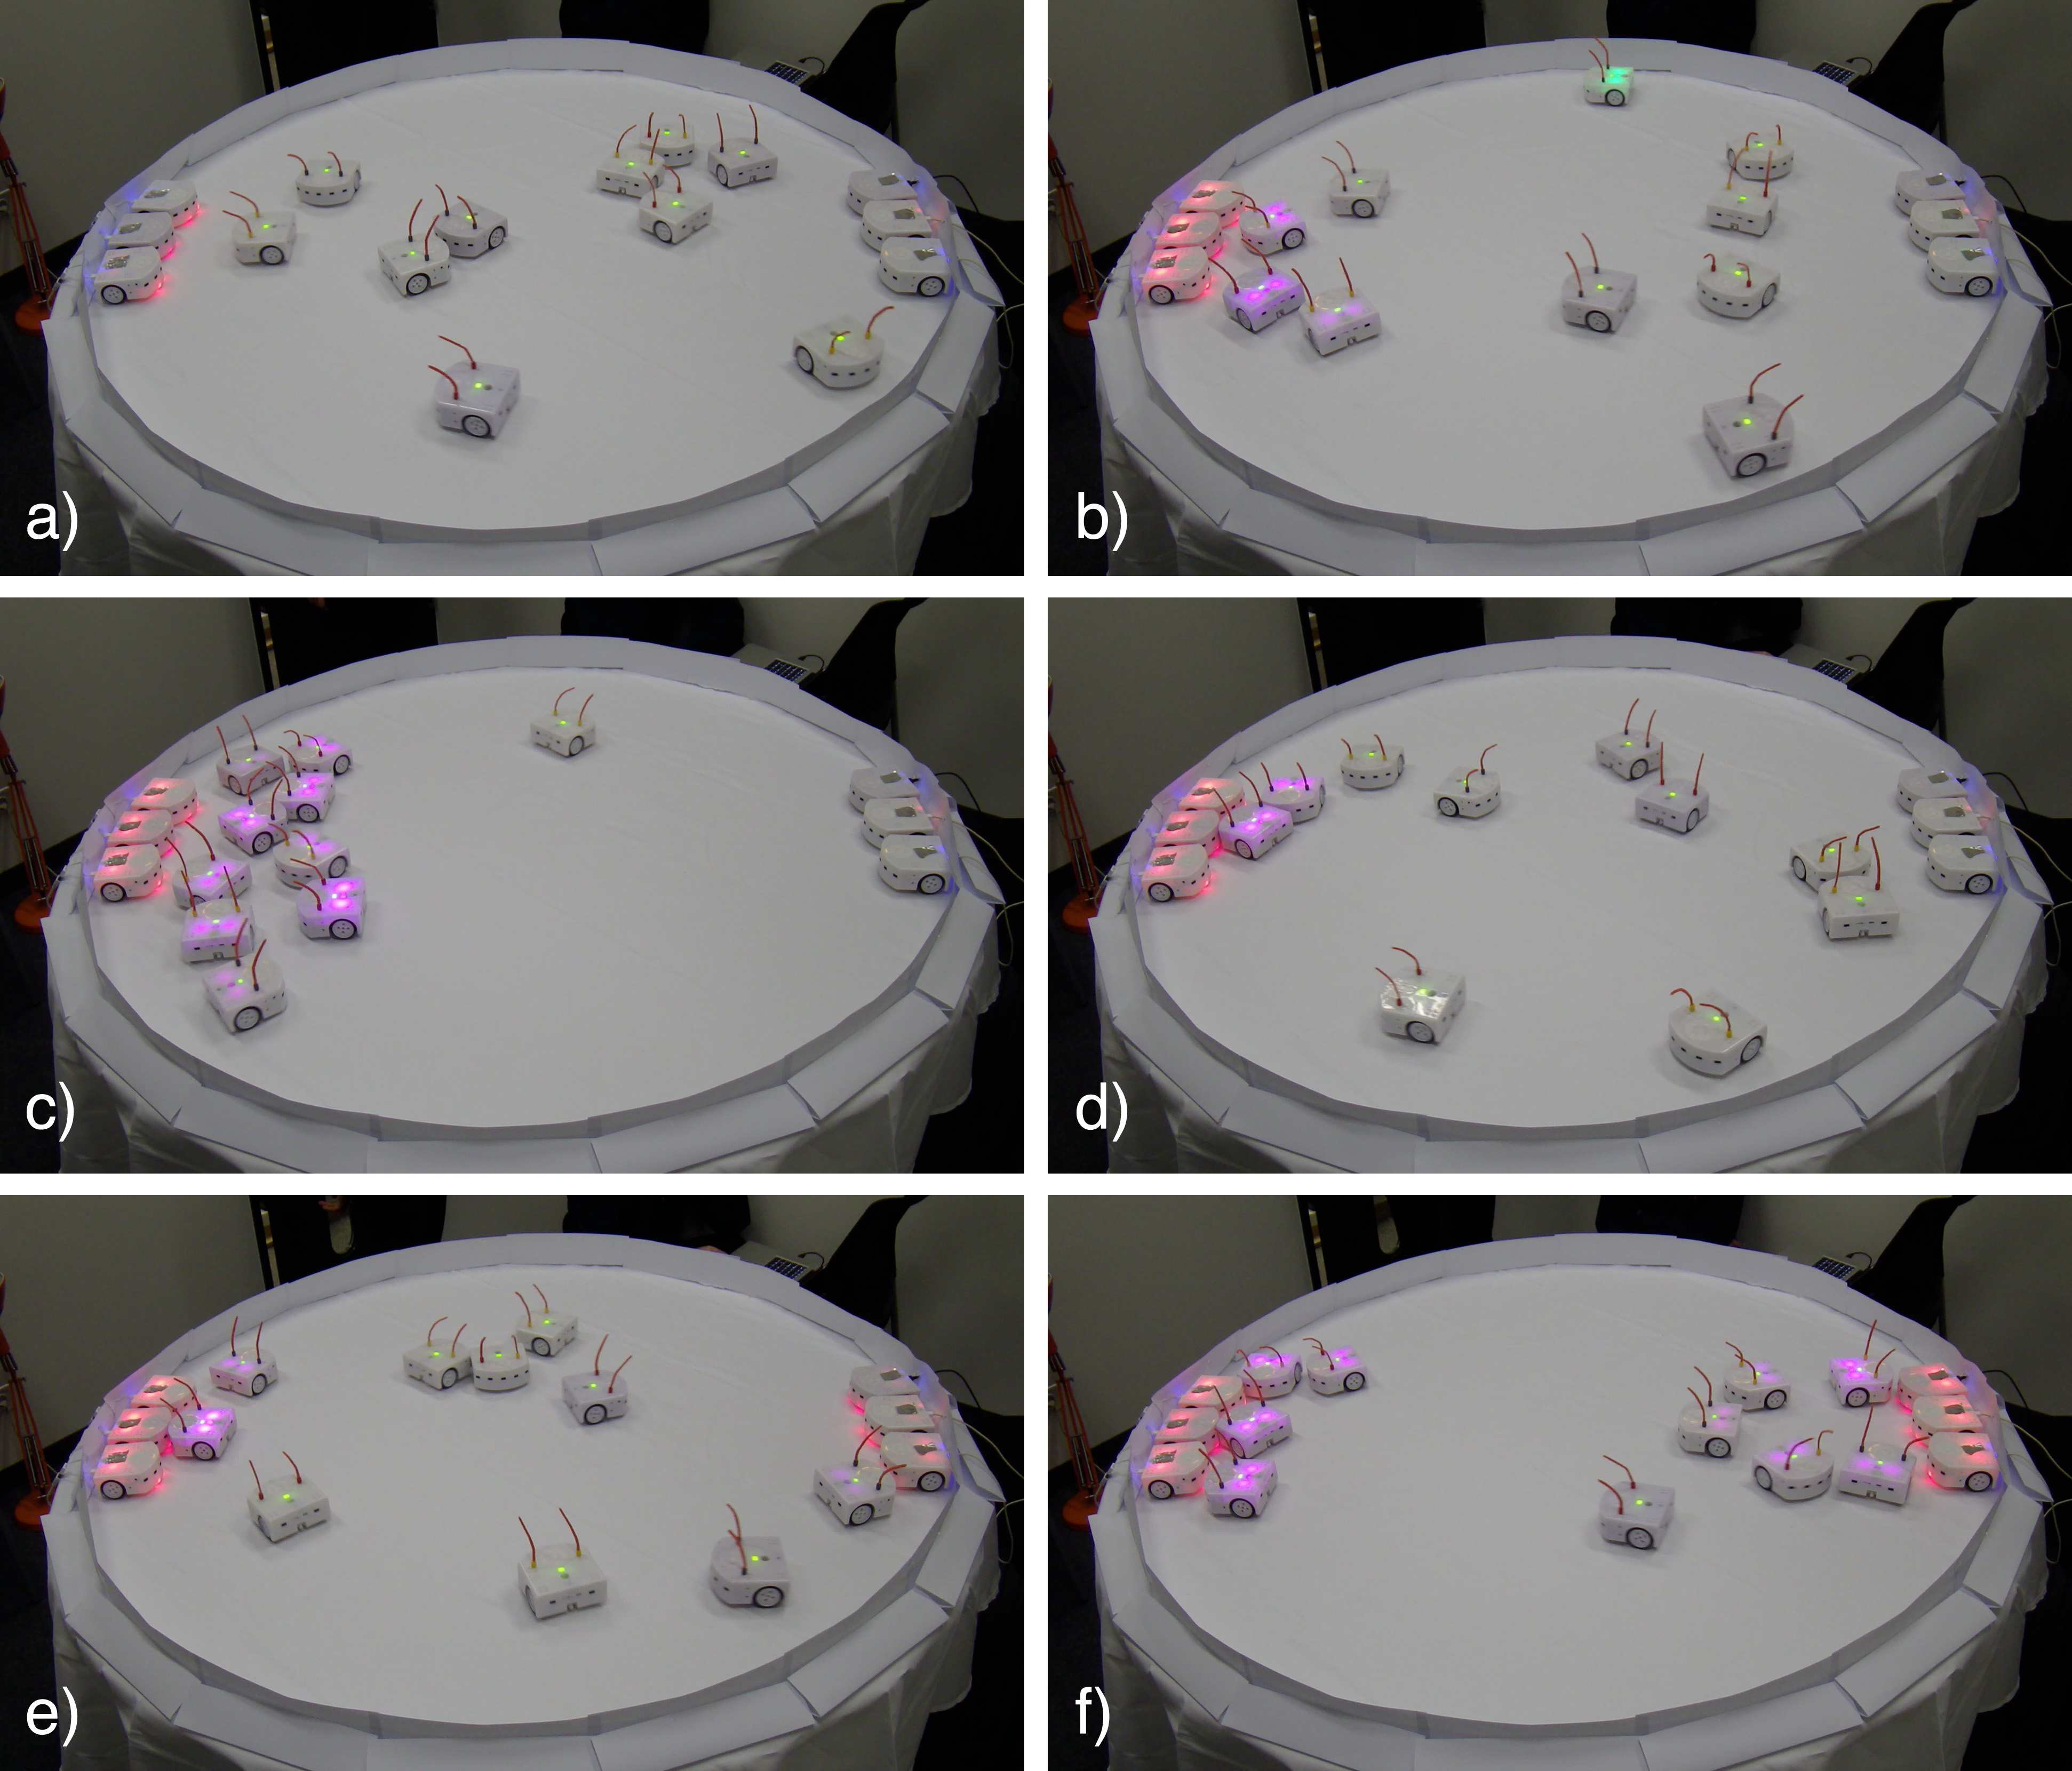
\includegraphics[width=\textwidth]{bee-clust}
\end{center}
\caption{Implementação do BeeClust. As fotografias foram tiradas nos seguintes momentos (minutos:segundos) desde o início da experiência: a) 1:40, b) 2:30, c) 9:40, d) 12:40, e) 13:20, f) 21:10.}\label{fig.beeclust-demo}
\end{figure}

Os três robôs emissores de calor do lado esquerdo transmitem sua temperatura. Os robôs apícolas nas proximidades detectam este sinal e param por um período de tempo proporcional à temperatura. Durante sua permanência nesta área, eles também transmitem um sinal de temperatura. Além disso, se os robôs emissores de calor detectarem robôs nas proximidades, eles aumentam seu calor e transmitem a nova temperatura. A figura~\ref{fig.beeclust-demo} mostra a evolução do comportamento dos robôs: (a) o estado inicial quando os robôs começam a se mover e somente a fonte de temperatura esquerda está ligada; (b) os robôs começam a se aglomerar em torno da fonte esquerda; (c) o mais alto nível de aglomeração ocorre. Os robôs-robôs podem deixar o aglomerado, explorar o ambiente e retornar ao aglomerado como mostrado em (d). Isto é causado pela natureza aleatória do algoritmo e é essencial para evitar que o sistema fique preso em mínimos locais. A Figura~\ref{fig.beeclust-demo}~(e) mostra o momento em que a fonte correta também é ligada. Após cerca de $21$ minutos, os robôs formam dois grupos menores (f).

\begin{framed}
\act{Algoritmo BeeClust}{beeclust-swarm-act}
\begin{itemize}
\item Implementar o algoritmo BeeClust para fazer com que um grupo de robôs se aglomere no local mais brilhante de uma sala.
\item Utilizar três sensores: um sensor de luz para medir a luz ambiente, um sensor para detectar outros robôs e um sensor para detectar os limites da arena.
\item Solução 1: Use sensores de proximidade para detectar outros robôs e sensores terrestres para detectar uma linha que defina os limites da arena.
\item Solução 2: Definir os limites da arena com uma parede e usar comunicações robô-robô para distinguir entre robôs e a parede. Para evitar confusão, não usar o mesmo sensor para detectar os outros robôs e a parede.
\end{itemize}
\end{framed}

\section{Robótica de enxame baseada em interações físicas}\label{s.swarm-physical}

Em Sect.~\ref{s.no-localization} olhamos para um exemplo típico de comportamento eficiente de enxame: uma colônia de formigas encontrando um caminho desde seu ninho até uma fonte de alimento. Esse exemplo utilizou comunicações indiretas na forma de feromônios depositados no solo. Nesta seção, olhamos para outra forma de comportamento de enxame que é mediada por interações físicas. Começamos com a colaboração de formigas na tarefa de puxar um pau do chão e uma versão robótica desta tarefa. Isto é seguido por uma discussão de como as forças exercidas por vários robôs podem ser combinadas, demonstradas por um algoritmo simples, mas inteligente chamado empurrão coletivo baseado na oclusão.

\subsection{Colaborando em uma tarefa física}

A figura~\ref{fig.real-ants-pulling} mostra duas formigas extraindo um bastão do chão para uso na construção de um ninho. A vara está embutida tão profundamente que uma formiga não consegue extraí-la sozinha. Queremos projetar um sistema robótico para realizar esta tarefa (Fig.~\ref{fig.robots-pulling}). Cada robô procura aleatoriamente até encontrar uma vara. Em seguida, ele puxa o bastão com a maior força possível. Se ele extrair a vara com sucesso, ele a leva de volta a um ninho; caso contrário, como ele extraiu apenas parcialmente a vara, ele espera até sentir que outro robô está puxando com mais força e solta a vara. Se nenhum robô vier em seu auxílio por um período de tempo, o robô libera seu porão e retorna a uma busca aleatória. Isto assegura que se houver mais varas do que robôs, o sistema não vai bloquear com cada robô tentando extrair uma vara e esperando indefinidamente.
\begin{figure}
\begin{minipage}{.45\textwidth}
\includegraphics[width=.45\textwidth]{real-ants-pulling}
\caption{Formigas puxando um pau do chão}
\label{fig.real-ants-pulling}
\end{minipage}
\hspace{\fill}
\begin{minipage}{.45\textwidth}
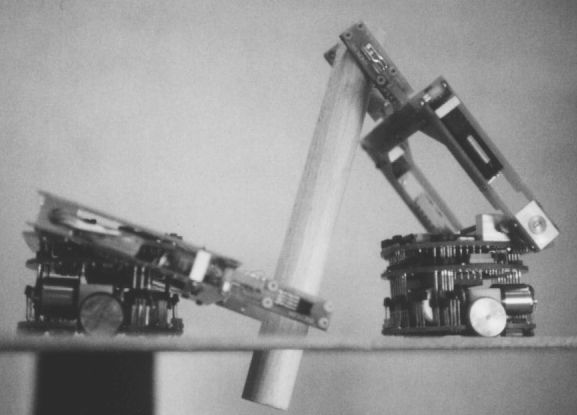
\includegraphics[width=.45\textwidth]{robots-pulling}
\caption{Robôs puxando um bastão do chão}
\label{fig.robots-pulling}
\end{minipage}
\end{figure}

%\begin{figure}
%\subfigures
%\begin{minipage}{\textwidth}
%\leftfigure{
%\includegraphics[width=.45\textwidth]{real-ants-pulling}
%}
%\hspace{\fill}
%\rightfigure{
%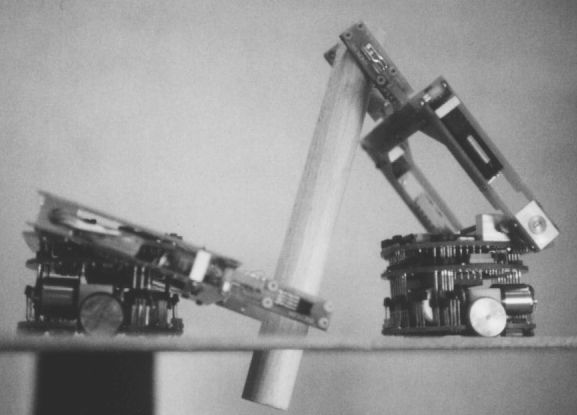
\includegraphics[width=.45\textwidth]{robots-pulling}
%}
%\leftcaption{Ants pulling a stick from the ground}\label{fig.real-ants-pulling}
%\rightcaption{Robots pulling a stick from the ground}\label{fig.robots-pulling}
%\end{minipage}
%\end{figure}

A máquina de estado finito para este algoritmo é mostrada na Fig.~\ref{fig.antspulling-FSM}. Embora este comportamento seja simples e local, quando aplicado por dois robôs, resulta na extração do bastão do solo. O robô à direita na Fig.~\ref{fig.antspulling-FSM} puxa parte da vara para fora do solo, utilizando o máximo movimento de seu braço. Quando detecta que outro robô encontrou a mesma vara e começa a puxá-la, o primeiro robô libera a vara para permitir que o segundo robô a extraia. Ao combinar a capacidade física de dois robôs com uma simples especificação de comportamento, obtemos um resultado que nenhum dos robôs conseguiria sozinho.

\begin{figure}
\begin{center}
\begin{tikzpicture}[node distance = 2.5cm and 50mm,align=left,minimum size=14mm,every loop/.style={min distance=16mm}]
% Nodes
\node[draw,circle] (looking) {\p{pesquisando}};
\node[draw,circle] (lifting) [right=of looking] {\p{levantamento}};
\node[draw,circle] (to-home) [below=of lifting] {\p{trazendo}\\\p{para aninhar-se}};
\node[draw,circle] (waiting) [below=of looking] {\p{esperando}};
% Initial state arrow
\draw[->] (-10mm,10mm) to node [above,yshift=0mm] {\p{verdadeiro} $\leadsto$\\\p{fwd, definir temporizador de busca}} (looking);
% Transitions from searching
\path[->] (looking) edge [loop left] node [below,yshift=-2mm] {\p{tempo limite de busca} $\leadsto$\\\p{virar aleatoriamente,}\\\p{fwd}} ();
\path[->] (looking) edge node[above,xshift=-2mm,yshift=-5mm] {\p{encontrado} $\leadsto$  \p{agarrar e levantar}} (lifting);
% Transitions from lifting
\path[->] (lifting) edge node[right] {\p{extraído} $\leadsto$\\ \p{ir para o ninho}} (to-home);
\path[->,bend left=10] (lifting) edge node[above,yshift=4mm,xshift=3mm] {\p{elevação máxima alcançada,}\\\p{não extraído} $\leadsto$\\\p{definir temporizador de espera}} (waiting);
% Transitions from to nest
\path[->,bend left=10] (to-home) edge node[left,yshift=-12mm,xshift=20mm] {\p{no ninho} $\leadsto$} (looking);
% Transitions from waiting
\path[->,bend right=20] (waiting) edge node[right] {\p{esperar}\\\p{tempo esgotado} $\leadsto$} (looking);
\path[->,bend left=20] (waiting) edge node[left,yshift=-8pt] {\p{outro robô}\\\p{puxando} $\leadsto$ \\\p{release the stick}} (looking);
\end{tikzpicture}
\end{center}
\caption{Algoritmo para puxar o bastão distribuído}\label{fig.antspulling-FSM}
\end{figure}

\subsection{Combinando as forças de vários robôs}

Fig~\ref{fig.pulling1} mostra um robô de acionamento diferencial movendo-se para trás (da esquerda para a direita). Ele exerce uma força de $F_r$ que pode ser usada para puxar um objeto. A figura~\ref{fig.pulling2} mostra dois robôs conectados entre si para que eles exerçam uma força $F_{\sub{total}}$ ao se moverem da esquerda para a direita.

\begin{figure}
\begin{center}
\begin{tikzpicture}
\pic[scale=.7] at (0,0) { robot-side };
\draw[->,thick] (-1.6,.7) -- node[above left] {$F_r$} (1,.7);
\end{tikzpicture}
\caption{Um robô puxando com uma determinada força $F_r$}\label{fig.pulling1}
\end{center}
\end{figure}

\begin{figure}
\begin{center}
\begin{tikzpicture}[scale=.6]
\pic[rotate=-20,scale=.7] at (0,0) { robot-side };
\pic[rotate=-20,scale=.7] at (8.5,-.4) { robot-side };
\draw[->,thick] (-1.3,0.8) -- node[above left] {$F_{\textit{total}}$} (1,0.8);
\draw[fill,gray!60] (62mm,2mm) -- ++(70:7mm) -- ++(-20:10mm) -- ++(70:25mm) -- ++(-20:25mm) -- ++(-110:6.3mm) -- ++(160:19mm) -- ++(-110:26mm) -- cycle;
\path (13,-3) rectangle ++(1,-3mm);  % Dummy for extra space
\end{tikzpicture}
\caption{Dois robôs conectados puxando com uma determinada força $F_{total}$}\label{fig.pulling2}
\end{center}
\end{figure}

Qual é a relação entre $F_r$ e $F_{\sub{total}}$? Há três possibilidades:
\begin{itemize}
\item $F_{\sub{total}} < 2 F_r$: Os robôs conectados perdem eficiência porque a força que exercem é menor do que a exercida pelos dois robôs que puxam separadamente.
\item $F_{\sub{total}} = 2 F_r$: Os robôs conectados atingem a mesma eficiência que dois robôs separados.
\item $F_{\sub{total}} > 2 F_r$: Os robôs conectados são mais eficientes do que dois robôs separados.
\end{itemize}
Os robôs podem conseguir $F_{\sub{total}} > 2 F_r$, onde a força total é maior que a soma das forças exercidas pelos robôs individuais, pois em algumas configurações mecânicas os robôs conectados são mais estáveis desde seu centro de gravidade melhor posicionados. 

\begin{framed}
\act{Força de tração por vários robôs}{pulling_force}
\begin{itemize}
\item Conecte dois robôs e verifique se eles exercem uma força menor, igual ou maior do que duas vezes a exercida por um único robô. Você pode conectar os robôs com uma conexão rígida como na Fig.~\ref{fig.pulling2} ou com uma conexão flexível usando fio.
\item Medir $F_r$, a força exercida por um único robô, e depois medir $F_{\sub{total}}$ a força exercida pelos robôs conectados.
\item Um \emph{dinamômetro} (Fig~\ref{fig.dyna}) é o melhor instrumento para medir forças. Se você não tiver um disponível, você pode usar um cabo, uma polia e pesos (ou uma balança) como mostrado na Fig.~\ref{fig.scale}.
\item Mudar a orientação dos robôs: puxando para frente ao invés de para trás. Isto muda o resultado?
\item Experimentar em diferentes superfícies (solo duro, tapete, papel) e determinar o efeito da superfície sobre a força resultante.
\end{itemize}
\end{framed}

\begin{figure}
\begin{center}
\begin{tikzpicture}[scale=.8]
% Table
\draw[fill,gray] (-6,-7.2mm) rectangle +(12,2mm);
\draw[fill,gray] (-5,-7.2mm) rectangle +(4mm,-4mm);
\draw[fill,gray] (5,-7.2mm) rectangle +(4mm,-4mm);
% Robot
\pic[scale=.6] at (0,0) { robot-side };
\draw[->,thick] (3.7,.7) -- node[above] {$F_r$} (6,.7);
% Attachment
\draw (-3,8mm) rectangle +(2,4mm);
\draw (-1,1) -- (0,1);
% Spring
\draw (-20mm,14mm) -- (-50mm,14mm) -- (-50mm,6mm) -- (-20mm,6mm);
\draw (-50mm,10mm) -- (-60mm,10mm);
\draw (-50mm,10mm) -- ++(2mm,2mm) -- ++(2mm,-4mm) -- ++(2mm,4mm)  -- ++(2mm,-4mm) -- ++(2mm,4mm)  -- ++(2mm,-4mm) -- ++(2mm,4mm)  -- ++(2mm,-4mm) -- ++(2mm,4mm)  -- ++(2mm,-3mm);
\end{tikzpicture}
\caption{Medindo a força com um dinamômetro}\label{fig.dyna}
\end{center}
\end{figure}

\begin{figure}
\begin{center}
\begin{tikzpicture}
% Table
\draw[fill,gray] (-2,-9mm) rectangle +(8,2mm);
\draw[fill,gray] (-1,-9mm) rectangle +(4mm,-15mm);
\draw[fill,gray] (5,-9mm) rectangle +(4mm,-15mm);
% Robot
\pic[scale=.6] at (0,-2.7mm) { robot-side };
\draw[->,thick] (3,.3) -- node[above] {$F_r$} (6,.3);
% Attachment
\draw[fill,gray!80] (-3,1mm) circle[radius=3mm];
\draw (-2.9,1mm) -- (-3.1,1mm);
\draw (-3,0mm) -- (-3,2mm);
\draw (-3,.4) -- (0,.4);
\draw (-33mm,2mm) -- ++(0,-19mm);
\draw[fill,gray!80] (-35mm,-16mm) rectangle +(4mm,4mm);
\draw (-40mm,-24mm) rectangle +(14mm,8mm);
\draw (-33mm,-20mm) circle[radius=3mm];
\draw[->] (-33mm,-20mm) -- +(30:3mm);
\end{tikzpicture}
\caption{Medindo a força com um peso e uma balança}\label{fig.scale}
\end{center}
\end{figure}

\subsection{Empurrão coletivo baseado na oclusão}

Consideremos outro exemplo de combinação da força de vários robôs. Em vez de uma ligação física como na Fig.~\ref{fig.pulling2}, usamos muitos robôs simples para empurrar um objeto, imitando um grupo de formigas. Mais uma vez, as vantagens de um sistema distribuído são a flexibilidade - empregando apenas os recursos necessários para a tarefa - e a robustez - se um robô falhar, o objeto pode se mover um pouco mais lentamente, mas o fracasso completo da tarefa não ocorre. Estas vantagens vêm ao custo de recursos adicionais e da complexidade de implementar a coordenação entre os robôs.

A figura~\ref{fig.swarm-pushing} mostra um grupo de pequenos robôs empurrando um objeto grande representado pelo círculo em direção a um objetivo. Uma abordagem seria determinar a direção para o objetivo, compartilhar esta informação entre todos os robôs e fazer com que cada robô compute a direção que deve empurrar. Isto não é tão simples quanto parece, já que um simples robô pode não ser capaz de determinar sua posição e direção absoluta.

Uma abordagem robótica de enxame é chamada de \emph{occlusion-based pushing}, que assume que os robôs têm apenas conhecimento local, não conhecimento global do que os outros robôs estão fazendo. Os robôs são capazes de determinar se eles podem ou não detectar o objetivo. Por exemplo, uma luz brilhante poderia ser montada sobre a meta e os robôs equipados com um sensor de luz. 

\begin{figure}
\begin{center}
\begin{tikzpicture}[scale=1.1]
\node[circle,draw,thick] (center) at (0,0) [minimum size=40mm] {};
\coordinate (goal) at (6,1.5);
\draw[fill] (goal) circle [radius=1pt];
\draw[->,shorten >= 50mm] (0,0) -- (goal);
\node at (6.5,1.5) {\p{goal}};
% Use negative shorten arrow trick to extend the tangent lines
\draw[shorten >= -50mm] (goal) -- (tangent cs:node=center, point={(goal)}, solution=1);
\draw[shorten >= -50mm] (goal) -- (tangent cs:node=center, point={(goal)}, solution=2);
% Draw the pushing robots
\foreach \angle/\x/\y in { 0/0mm/0mm, -20/2mm/10mm, -40/7mm/18mm, 20/2mm/-10mm, 40/7mm/-18mm, 60/14mm/-22mm } {
  \pic[rotate=\angle,scale=0.3] at (\x-24mm, \y) { robot };
  \draw[->] (\x-24mm,\y) -- +(\angle:8mm);
}
% Draw the non-pushing robots
\pic[rotate=-80,scale=0.3] at (0mm, 28mm) { robot };
\path[->,bend right=40,red,thick] (0mm,28mm) edge (8mm,26mm);
\pic[rotate=60,scale=0.3] at (8mm, -28mm) { robot };
\path[->,bend left=30,red,thick] (8mm,-28mm) edge (16mm,-24mm);
\pic[rotate=-120,scale=0.3] at (30mm, 10mm) { robot };
\path[->,bend right=50,red,thick] (30mm,10mm) edge (36mm,4mm);
\end{tikzpicture}
\end{center}
\caption{Coordenação baseada na oclusão: setas negras retas para os robôs empurrando o objeto e setas vermelhas curvas para os robôs em busca de uma posição ocluída}\label{fig.swarm-pushing}
\end{figure}

A figura~\ref{fig.FSM-swarm-pushing} mostra a máquina de estado finito para este algoritmo. Os robôs procuram o objeto; quando o encontram, eles se colocam perpendicularmente à superfície e empurram (setas negras retas). Isto pode ser implementado usando um sensor de toque ou um sensor de proximidade. Os robôs continuam a empurrar enquanto não detectam o objetivo. Se detectarem a meta, eles param de empurrar, se afastam (setas vermelhas curvas) e iniciam uma nova busca por uma posição ocluída onde eles retomam o empurrão. O resultado é que a soma vetorial das forças exercidas pelos robôs está em uma direção que move o objeto em direção ao objetivo. O algoritmo de oclusão leva a tarefa a ser executada sem uma unidade central de controle e até mesmo sem comunicações entre robôs.

\begin{figure}
\begin{center}
\begin{tikzpicture}[node distance = 4cm and 5cm,align=left,minimum size=16mm,every loop/.style={min distance=16mm}]
% Nodes
\node[draw,circle] (searching) {\p{searching}\\\p{for object}}; and their fit to the required performances of the system.
\node[draw,circle] (pushing) [right=of searching] {\p{pushing}};
% Initial state arrow
\draw[->] (-5mm,12mm) to node [above left,yshift=-2mm,xshift=6mm] {\p{true} $\leadsto$\\\p{move randomly}} (searching);
% Transitions from searching
\path[->,bend left=30] (searching) edge node [above,yshift=-4mm] {\p{object found and goal occluded} $\leadsto$\\\p{push object}} (pushing);
% Transitions from pushing
\path[->] (pushing) edge [loop right] node[below,xshift=-2mm] {\p{goal occluded} $\leadsto$} (pushing);
\path[->,bend left=30] (pushing) edge node[below,yshift=4mm] {\p{goal visible} $\leadsto$\p{move randomly}} (searching);
\path[->] (pushing) edge node[above,yshift=-6mm] {\p{object lost} $\leadsto$\p{move randomly}} (searching);
\end{tikzpicture}
\end{center}
\caption{Algoritmo para a coordenação baseada na oclusão}\label{fig.FSM-swarm-pushing}
\end{figure}

\begin{framed}
\act{Força total}{total-force}
\begin{itemize}
\item Considere a configuração mostrada na Fig.~\ref{fig.total-force}. O robô $1$ está empurrando um objeto a um ângulo de $45^{\circ}$ com força $f_1$, o robô $2$ está empurrando horizontalmente com força $f_2$ e o robô $3$ está empurrando verticalmente com força $f_3$. Mostrar que o $f_{\sub{total}}$, a força total sobre o objeto, tem magnitude:
\[
\sqrt{\left(f_2+\frac{f_1}{\sqrt{2}}\right)^2+\left(f_3-\frac{f_1}{\sqrt{2}}\right)^2}\,.
\]
na direção:
\[
\alpha = \tan^{-1} \frac{2f_3-\sqrt{2}f_1}{2f_2+\sqrt{2}f_1}\,.
\]
\item Calcule a magnitude e a direção de $f_{\sub{total}}$ para vários valores das forças individuais. Se $f_1=f_2=f_3=1$, a magnitude é de $\sqrt{3}$ e a direção é de $9,7^{\circ}$. Se $f_1=f_2=1$, o que deve ser $f_3$ para que $f_3$ seja $f_45^{\circ}$?
\item Usar três robôs para implementar esta configuração e verificar se o objeto se move na direção computada.
\end{itemize}
\end{framed}


\begin{figure}
\begin{center}
\begin{tikzpicture}[scale=1.2]
\draw[fill] (0,0) circle [radius=4pt];
\draw[->] (-3,0) -- node[above,near start] {$f_2$} (-4pt,0);
\draw[->] (0,-2) -- node[left,near start] {$f_3$} (0,-4pt);
\draw[->] (-45:-3) -- node[above,near start,yshift=4pt] {$f_1$} (-2pt,2pt);
\draw (-10mm,0) arc (180:135:10mm) node[midway,xshift=-3mm,yshift=1mm] {$45^{\circ}$};
\draw[dashed] (0,0) -- (3,0);
\draw[->] (0,0) -- node[above,near end,xshift=-1mm] {$f_{\sub{total}}$} (20:3);
\draw (15mm,0) arc (0:20:15mm) node[right,midway] {$\alpha$};
\end{tikzpicture}
\caption{A força total de três robôs}\label{fig.total-force}
\end{center}
\end{figure}

\begin{framed}
\act{Empurrando com base na oclusão}{occulsion-swarm}
\begin{itemize}
\item Coloque três robôs ao redor de um objeto e coloque uma meta a alguma distância do robô. Implemente um mecanismo para que os robôs determinem a direção para a meta, por exemplo, prenda uma luz à meta ou coloque a meta no ponto mais baixo de uma superfície inclinada.
\item Implementar um mecanismo que permita aos robôs distinguir entre o objeto e o limite da superfície na qual eles se movem. Por exemplo, usar uma fita preta na superfície para seu limite e detectar o objeto usando sensores de proximidade.
\item Implementar um mecanismo para que os robôs não se empurrem uns aos outros. Um método seria usar um sensor colorido e prender fita adesiva colorida aos robôs.
\item Implementar o algoritmo de empurrar baseado na oclusão.
\item Discutir se o empurrão baseado na oclusão poderia ser usado em três dimensões, por exemplo, robôs subaquáticos empurrando um objeto.
\end{itemize}
\end{framed}

\section{Sumário}

A robótica de enxame usa vários robôs em uma arquitetura distribuída para realizar uma tarefa. Com uma arquitetura distribuída, o sistema é robusto à falha de robôs individuais e flexível em sua capacidade de adicionar ou remover robôs à medida que a escala da tarefa muda. Uma arquitetura distribuída pode executar tarefas que robôs individuais não podem, como vimos nos exemplos de robôs que combinam forças. Finalmente, vários robôs podem agir simultaneamente em locais diferentes que estão longe uns dos outros. Estas vantagens têm um preço: o aumento do custo dos múltiplos robôs, a complexidade dos mecanismos de coordenação que devem ser implementados e, em alguns casos, a perda de desempenho devido à sobreposição da ação de diferentes robôs. 

\section{Leitura adicional}

Uma visão geral da robótica coletiva é dada no manual \cite{kernbach2013} e a coleção \cite{sahin2005} se concentra na robótica de enxame. Para os projetos específicos apresentados neste capítulo, veja:
\begin{itemize}
\item Karel the Robot~\cite{karel}.
\item BeeClust~\cite{bodi2012interaction} and~\cite{Schmickl2009}.
\item ASSISIbf~\cite{schmickl2013assisi} and \url{http://assisi-project.eu}.
\item Physical interaction (pulling a stick)~\cite{Ijspeert2001}.
\item Occlusion-based transport~\cite{chen2013strategy} and \cite{gross2015}.
\end{itemize}
